\documentclass[10pt,a4paper]{article}
\usepackage[utf8]{inputenc}
\usepackage{amsmath}
\usepackage{amsfonts}
\usepackage{amssymb}
\usepackage{mathtools}
\usepackage{bm}
\newcommand\bigzero{\makebox(0,0){\text{\large 0}}}
\usepackage{graphicx}
\usepackage{epstopdf} 
\usepackage[justification=centering]{subfig}
\usepackage[T1]{fontenc}
\usepackage{lmodern}


\newcommand{\vectornorm}[1]{\left\|#1\right\|}

\newcommand{\threepartdef}[6]
{
	\left\{
		\begin{array}{lll}
			#1 & \mbox{for } #2 \\
			#3 & \mbox{for } #4 \\
			#5 & \mbox{for } #6
		\end{array}
	\right.
}

\begin{document}
\title{Semester project}
\author{Espen Johansen Velsvik}
\maketitle

\section{Motivation}
When an observer of an object moves relative to the object, there is an apparent relative motion in the image plane of the observer. The problem of determining this relative motion from a sequence of images is called the Optical Flow problem. The analysis is not so much dependent on prior knowledge of the scene, but on the image sequence itself. This independency makes it applicable in many different fields. More concisely, one wants to find flow vector components $u,v \in \mathbb{R}$ by looking at the change in brightness $f(x,t)$ at a specific pixel from one frame to another for $x \in \Omega$, where $\Omega$ is considered to be a rectangular domain. This is problematic because we can not independently determine a vector of 2 components using one constraint coming from the change in image brightness at a point $x \in \Omega$. Thus we need to impose other constraints to make the problem solvable.

\section{The Brightness constancy assumption}
The starting point for the variational approach to optical flow is the so called brightness constancy assumption of Horn and Schunck \cite{HS}. Let $f(x,t)$ be the grayscale value of some image sequence. To constrain our problem we make an assumption regarding invariance in the brightness: a point moving with velocity $\frac{dx}{dt} = u(x,t)$ along the trajectory $x(t)$ over time $t$ does not change its appearance. This assumption is called the brightness constancy assumption, and it means that if the scene has the same lighting, then movement of an object along a trajectory does not change its brightness. In mathematical notation this is (under perfect conditions) equivalent to the following:
\begin{align*}
\frac{d}{dt}f(x(t),t) = 0.
\end{align*}
By using the chain rule for differentiation, and defining $\frac{dx}{dt} = u$ and $\frac{dy}{dt} = v$, one gets
\begin{align*}
\frac{\partial f}{\partial x} u + \frac{\partial f}{\partial y} v + \frac{\partial f}{\partial t} = 0,
\end{align*}
or equivalently $\nabla f \cdot (u,v) = \frac{\partial f}{\partial t}$. So from this equation we can only determine the components of the movement in the direction of the gradient, or what is known as the normal flow. This is called the Aperture problem, and to be able to compute the components of the flow vector one needs another constraint. Following the notation and terminology of \cite{OFH}, the constraint coming from the brightness constancy assumption is called the data term $M(u,v)$

\section{The Smoothness constraint}
The second constraint is referred to as the smoothness constraint. It says that points can not move independently in the brightness pattern. There has to be some smoothness in the flow vector for points belonging to the same object. In other words, points on the same object moves with the same velocity. A natural way of obtaining a smoother solution would be to minimize some term depending on the sizes of the gradients in some direction. For now we let this smoothness term be $V(\nabla u, \nabla v)$.

\section{The variational formulation}
To combine the two constraints into one term we form a global energy function consisting of the data term and the smoothness term:
\begin{align}
E(u,v) = \frac{1}{2} \int_\Omega (M(u,v) + \frac{1}{\sigma^2} V(\nabla u, \nabla v)) \, dx dy,
\end{align}
where $\sigma > 0$ is a regularization parameter. The problem is now to find the minimum of the energy functional $E(u,v)$. Let $\textbf{w} = (u,v)$. From calculus of variations we have that if $\textbf{w}$ minimizes a functional $J(\textbf{w}) = \iint \limits_\Omega F(x,y,\textbf{w},\textbf{w}_x,\textbf{w}_y) \, dxdy$ then the first variation must be zero:
\begin{align*}
\delta J(\textbf{w}) = \frac{d}{d \epsilon} \left[ J(\textbf{w} + \epsilon \bm{\eta}) \right] = 0 
\end{align*}
for any arbitrary function $\bm{\eta}(x,y)$. We get
\begin{align*}
\delta J(\textbf{w}) =&  \iint \limits_{\Omega} \frac{d}{d \epsilon} F(x,y,\textbf{w} + \epsilon \bm{\eta}, \textbf{w}_x + \epsilon \bm{\eta}_x, \textbf{w}_y + \epsilon \bm{\eta}_y) \, dxdy \\
=&  \iint \limits_{\Omega} \bm{\eta} F_\textbf{w} + \bm{\eta}_x F_{\textbf{w}_x} + \bm{\eta}_y F_{\textbf{w}_y} \, dxdy \\
=& \iint \limits_{\Omega} \bm{\eta} F_\textbf{w} + \frac{d}{d x} (\bm{\eta} F_{\textbf{w}_x}) + \frac{d }{d y} (\bm{\eta} F_{\textbf{w}_y}) - \bm{\eta} \left( \frac{d}{d x} F_{\textbf{w}_x} + \frac{d }{d y} F_{\textbf{w}_y} \right) \, dxdy
\end{align*}
Now let $\Gamma_{E}$, $\Gamma_{W}$, $\Gamma_{N}$ and $\Gamma_{S}$ be the east, west, north and south boundary of our domain respectively. Then using Gauss' Theorem gives
\begin{align*}
& \iint \limits_{\Omega}  \frac{d}{d x} (\bm{\eta} F_{\textbf{w}_x}) + \frac{d }{d y} (\bm{\eta} F_{\textbf{w}_y}) \, dxdy \\ =  &\int_{\Gamma_{e}} \bm{\eta} F_{\textbf{w}_x} \, dx - \int_{\Gamma_{w}} \bm{\eta} F_{\textbf{w}_x} \, dx + \int_{\Gamma_{n}} \bm{\eta} F_{\textbf{w}_y} \, dy - \int_{\Gamma_{s}} \bm{\eta} F_{\textbf{w}_y} \, dy
\end{align*}
Using this result, we get
\begin{align*}
&\delta J(\textbf{w}) = \iint \limits_{\Omega} \bm{\eta} \left( F_\textbf{w} -  \frac{d}{d x} F_{\textbf{w}_x} - \frac{d }{d y} F_{\textbf{w}_y} \right) \, dxdy  \\ + & \left( \int_{\Gamma_{E}} \bm{\eta} F_{\textbf{w}_x} \, dx - \int_{\Gamma_{W}} \bm{\eta} F_{\textbf{w}_x} \, dx + \int_{\Gamma_{N}} \bm{\eta} F_{\textbf{w}_y} \, dy - \int_{\Gamma_{S}} \bm{\eta} F_{\textbf{w}_y} \, dy \right) = 0.
\end{align*}
Since this must hold for any arbitrary function $\bm{\eta}(x,y)$ it follows that
\begin{align*}
F_{\textbf{w}} - \frac{d}{dx} F_{\textbf{w}_x} - \frac{d }{d y} F_{\textbf{w}_y} &= 0 \quad \text{in} \ \Omega \\
F_{\textbf{w}_x} &= 0 \quad \text{on} \ \Gamma_e \ \text{and} \ \Gamma_w \\
F_{\textbf{w}_y}& = 0 \quad \text{on} \ \Gamma_n \ \text{and} \ \Gamma_s
\end{align*}
This is called the Euler-Lagrange equation of variational calculus. From this result it is easy to see that the following must hold for our functional:
\begin{equation}
\label{EL}
  \begin{aligned}
\partial_{\textbf{w}} M - \frac{1}{\sigma^2}\left( \frac{d}{d x} \partial_{\textbf{w}_x} V + \frac{d}{d y} \partial_{\textbf{w}_y} V \right) &= 0 \quad \text{in} \ \Omega  \\
\partial_{\textbf{w}_x} V &= 0 \quad \text{on} \ \Gamma_E \ \text{and} \ \Gamma_W \\
\partial_{\textbf{w}_y} V &= 0 \quad \text{on} \ \Gamma_N \ \text{and} \ \Gamma_S
  \end{aligned}
\end{equation}
The smoothness term will be a function of the gradient of the flow. It is convenient to write the first equation in the Euler-Lagrange system in the form
\begin{equation}
\label{EL_regu}
  \begin{aligned}
\partial_q M - \frac{1}{\sigma^2} \text{div} \left(\Theta \nabla q \right) = 0 \\
	\end{aligned}
\end{equation}
for $q \in u, v$ where $\Theta$ is a diffusion matrix steering the direction of the diffusion, and can be both dependent or independent of the gradient itself. The framework above will be the same for all the methods explained below, and the choice of diffusion matrix will be the thing that separates them. 

\begin{table}
\begin{tabular}{c|c}
Method & $\Theta$
\end{tabular}
\caption{$log(\vectornorm{e^{(i)}}_{\infty n})$-values for the Jacobi algorithm }
\label{nvalues}
\end{table}

\section{The approach by Horn and Schunck}
The research of Horn and Shunck (1981) has formed the basis of further research in the field of optical flow. They proposed the following quadratic penalised data term
\begin{align}
M(\textbf{w}) = (\nabla f \textbf{w} + \frac{\partial f}{\partial t})^2 = (\frac{\partial f}{\partial x} u + \frac{\partial f}{\partial y} v + \frac{\partial f}{\partial t})^2,
\end{align}
where $\textbf{w} = (u,v)$. Most of the methods in variational optical flow use this data term. The contribution to (\ref{EL}) are the following two terms
\begin{equation}
\begin{aligned}
\frac{\partial M}{\partial u} = 2(\frac{\partial f}{\partial x}u + \frac{\partial f}{\partial y}v + \frac{\partial f}{\partial t}) \frac{\partial f}{\partial x} \\
\frac{\partial M}{\partial v} = 2(\frac{\partial f}{\partial x}u + \frac{\partial f}{\partial y}v + \frac{\partial f}{\partial t}) \frac{\partial f}{\partial y}. \\
\end{aligned}
\end{equation}

The smoothness term used by Horn and Schunck is the following
\begin{align*}
V(\nabla u, \nabla v) = |\nabla u|^2 + |\nabla v|^2.
\end{align*}
This is a homogeneous regularizer which means that it applies an equal amount of diffusion in all directions. In the framework of (\ref{EL_regu}), this is equivalent to the diffusion matrix $\Theta$ being the identity matrix. Using this function as a flow regularizer gives
\begin{align*}
\frac{\partial V}{\partial q_{x_i}} = 2q_{x_i},
\end{align*}
for $q \in u,v$ and $x_i = x, y$. Dividing by the factor of 2 in all terms results in (\ref{EL}) taking the form 
\begin{equation}
\label{EL_HS}
\begin{aligned}
(\frac{\partial f}{\partial x}u + \frac{\partial f}{\partial y}v + \frac{\partial f}{\partial t}) \frac{\partial f}{\partial x} - \frac{1}{\sigma^2}(\frac{\partial}{\partial x} \frac{\partial u}{\partial x} + \frac{\partial}{\partial y} \frac{\partial u}{\partial y} ) &= 0  \quad \text{in} \ \Omega,  \\
(\frac{\partial f}{\partial x}u + \frac{\partial f}{\partial y}v + \frac{\partial f}{\partial t}) \frac{\partial f}{\partial y} - \frac{1}{\sigma^2}(\frac{\partial}{\partial x} \frac{\partial v}{\partial x} + \frac{\partial}{\partial y} \frac{\partial v}{\partial y} ) &= 0  \quad \text{in} \ \Omega  \\
& \text{and} \\
\textbf{w}_{x} &= 0 \quad \text{on} \ \Gamma_e \ \text{and} \ \Gamma_w, \\
\textbf{w}_{y} &= 0 \quad \text{on} \ \Gamma_n \ \text{and} \ \Gamma_s.
\end{aligned}
\end{equation}



\subsection{Discretizing the Horn and Schunck method}
\label{sec: disc}
Let now our image be of dimension m-by-n, and let $f^1$ and $f^2$ be the image at $t=1$ an $t=2$ respectively. Also, we flatten the regular 2-dimensional grid in $\Omega$ and consider now $(x^i)_ {i \in [mn]}$ so that $(x,y) = (\left \lfloor{i/m}\right \rfloor, i - \left \lfloor{i/m}\right \rfloor) h$, with $h$ being the distance between vertical and horisontal grid points in $\Omega$. The corresponding vector representation of the image $f$ is denoted as $\textbf{f}(x^i) \in \mathbb{R}^{mn}$. Continuing this notation, the discrete flow values $\textbf{w}(x^i)$ is represented as the following vector in $\mathbb{R}^{2mn}$:
\begin{align*}
     \textbf{w}(x^i)=\begin{bmatrix}
         u(x^i)_{i\in [mn]}  \\
         v(x^i)_{i \in [mn]} \\
        \end{bmatrix}.
\end{align*}
For the discretization of the image gradients in (\ref{EL_HS}), the forward difference was used on $f^1$, producing the two vectors $\textbf{d}_x(x^i)$ and $\textbf{d}_y(x^i)$ in $\mathbb{R}^{mn}$. For the boundaries $\Gamma_E$ and $\Gamma_S$ a constant gradient was assumed. The time derivative $\frac{\partial f}{\partial t}$ is discretized using forward difference as shown below:
\begin{align*}
\textbf{c}(x^i) = \textbf{f}^2(x^i) - \textbf{f}^1(x^i),
\end{align*} 
where $\textbf{c}(x^i)$ is a vector in $\mathbb{R}^{mn}$. When choosing the derivative approximations for the flow vector in (\ref{EL_HS}), the first derivative was approximated using backward difference, and the second was approximated using forward difference. The resulting system to be solved is shown below:
\begin{align}
(D^T D + \frac{1}{\sigma^2} L^TL) \textbf{w} = - D^T \textbf{c}.
\end{align}
$D$ is the following block matrix:
\begin{align*}
D = \left[
\begin{array}{c|c}
D_x & D_y
\end{array}
\right],
\end{align*}
where $D_x$ and $D_y$ are diagonal matrices in $\mathbb{R}^{mn \times mn}$ with the elements of $\textbf{d}_x(x^i)$ and $\textbf{d}_y(x^i)$ along its diagonals respectively. $L$ is the following block matrix:
\begin{align*}
L = \left[
\begin{array}{c|c}
L_x & 0_{mn,mn} \\
L_y & 0_{mn,mn} \\
0_{mn,mn} & L_x \\
0_{mn,mn} & L_y \\
\end{array}
\right],
\end{align*}
$Lx \in \mathbb{R}^{mn \times mn}$ being the following mn-by-mn block diagonal matrix:
\begin{align*}
L_x = \left[
\begin{array}{c|c|c|c}
I_{m} & -I_{m} & 0 & \cdots \\ \hline
0 &  I_{m} & -I_{m} & 0 \\ \hline
0 & 0 & \ddots & \ddots \\
\end{array}
\right],
\end{align*}
and $L_y \in \mathbb{R}^{mn \times mn}$ the following band matrix:
\begin{align*}
L_y = \left[
\begin{array}{c c c c}
1 & -1 &  & \bigzero \\ 
 \bigzero & \ddots & \ddots &  \\
 &  & 1 & -1 \\
\end{array}
\right].
\end{align*}
The matrix multiplication with $L$ gives a forward difference approximation, and $-L^T$ gives a backward difference approximation. The matrix product $-L^TL$ is then the discretization of the second derivative in (\ref{EL_HS}).

\subsection{Results for the Horn and Schunck method}
The results when running the Horn and Schunck algorithm on our test images shown in Figures \ref{taxi1} and \ref{taxi2} for different regularization parameters are shown in Figure \ref{reguHS}. The choice of regularization parameter depends on the application, but one often want to get rid of most of the internal structure in each object, since these points will be moving with the same velocity (when assuming no deformation of the object). One also want to have a good enough balance between segmentation and smoothing. It is seen that choosing $\sigma = 0.003$ gives a fairly good segmentation of the objects that are moving, and with almost no internal structure. The flow field with this choice of regularization parameter is shown in Figure \ref{reguHS_best} on its own. The Horn and Schunck smoothes the flow in all directions, and the flow boundaries are therefore a bit smudged. 


\begin{figure}
\centering
\begin{minipage}{0.45\textwidth}
\centering
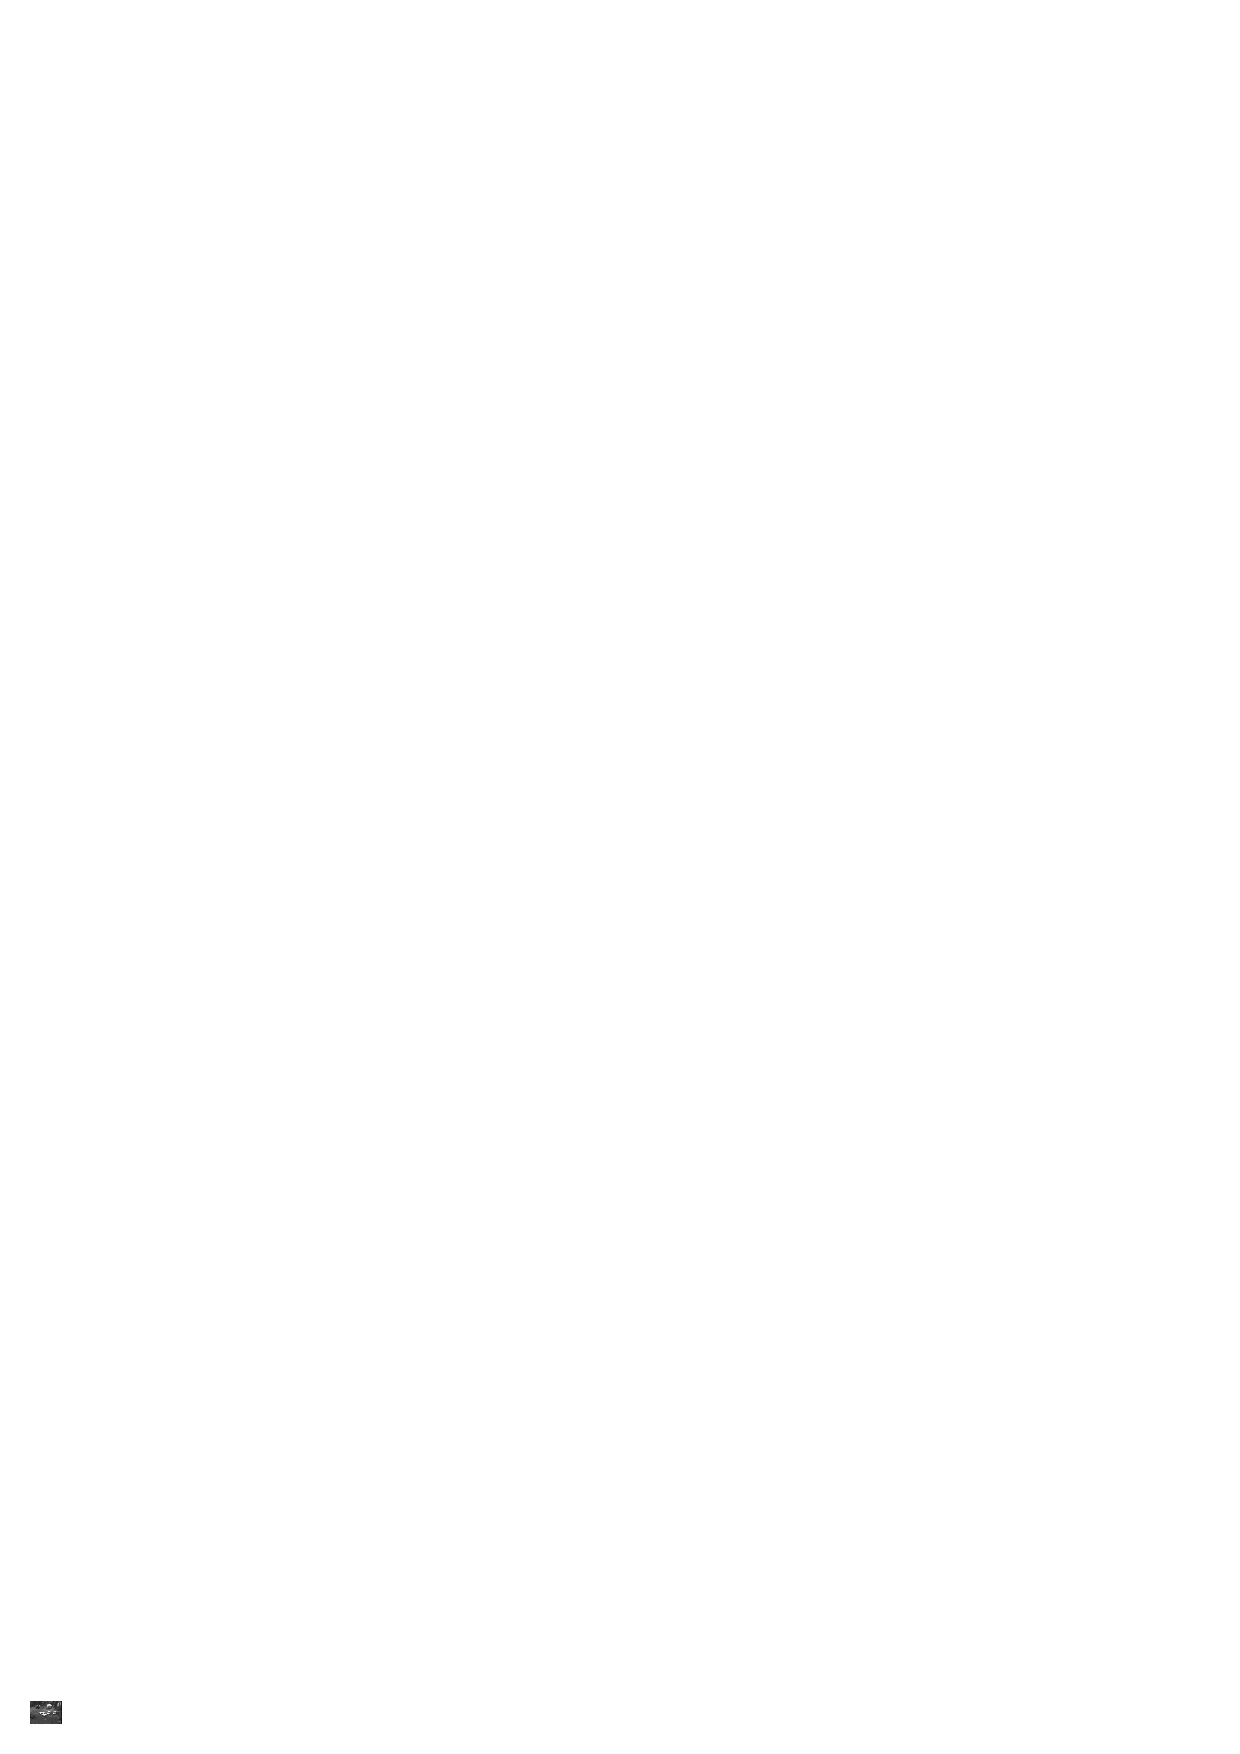
\includegraphics[scale=9]{taxi-00}
\caption{First image in the Hamburg taxi sequence.}
\label{taxi1}
\end{minipage}\hfill
\begin{minipage}{0.45\textwidth}
\centering
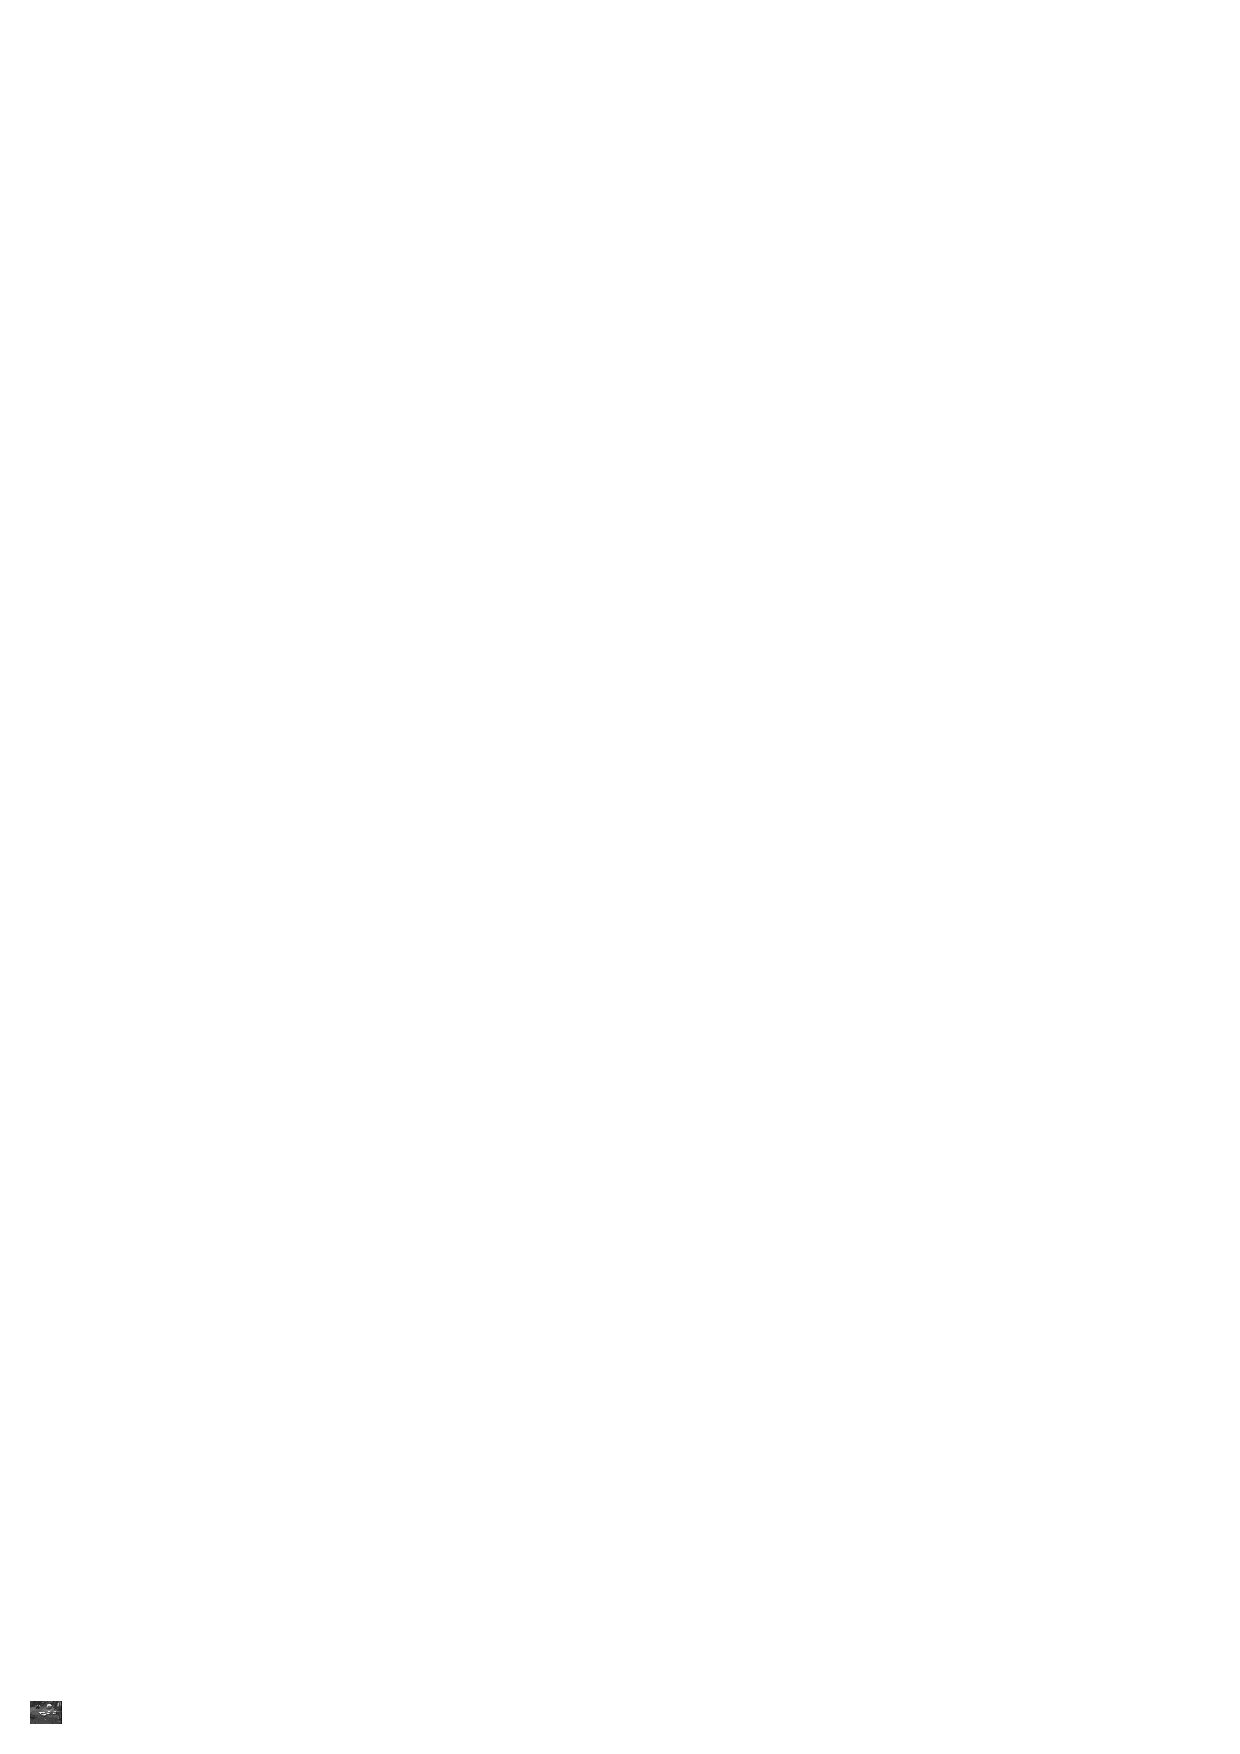
\includegraphics[scale=9]{taxi-01}
\caption{Second image in the Hamburg taxi sequence.}
\label{taxi2}
\end{minipage}
\end{figure}

\begin{figure}
    \centering
    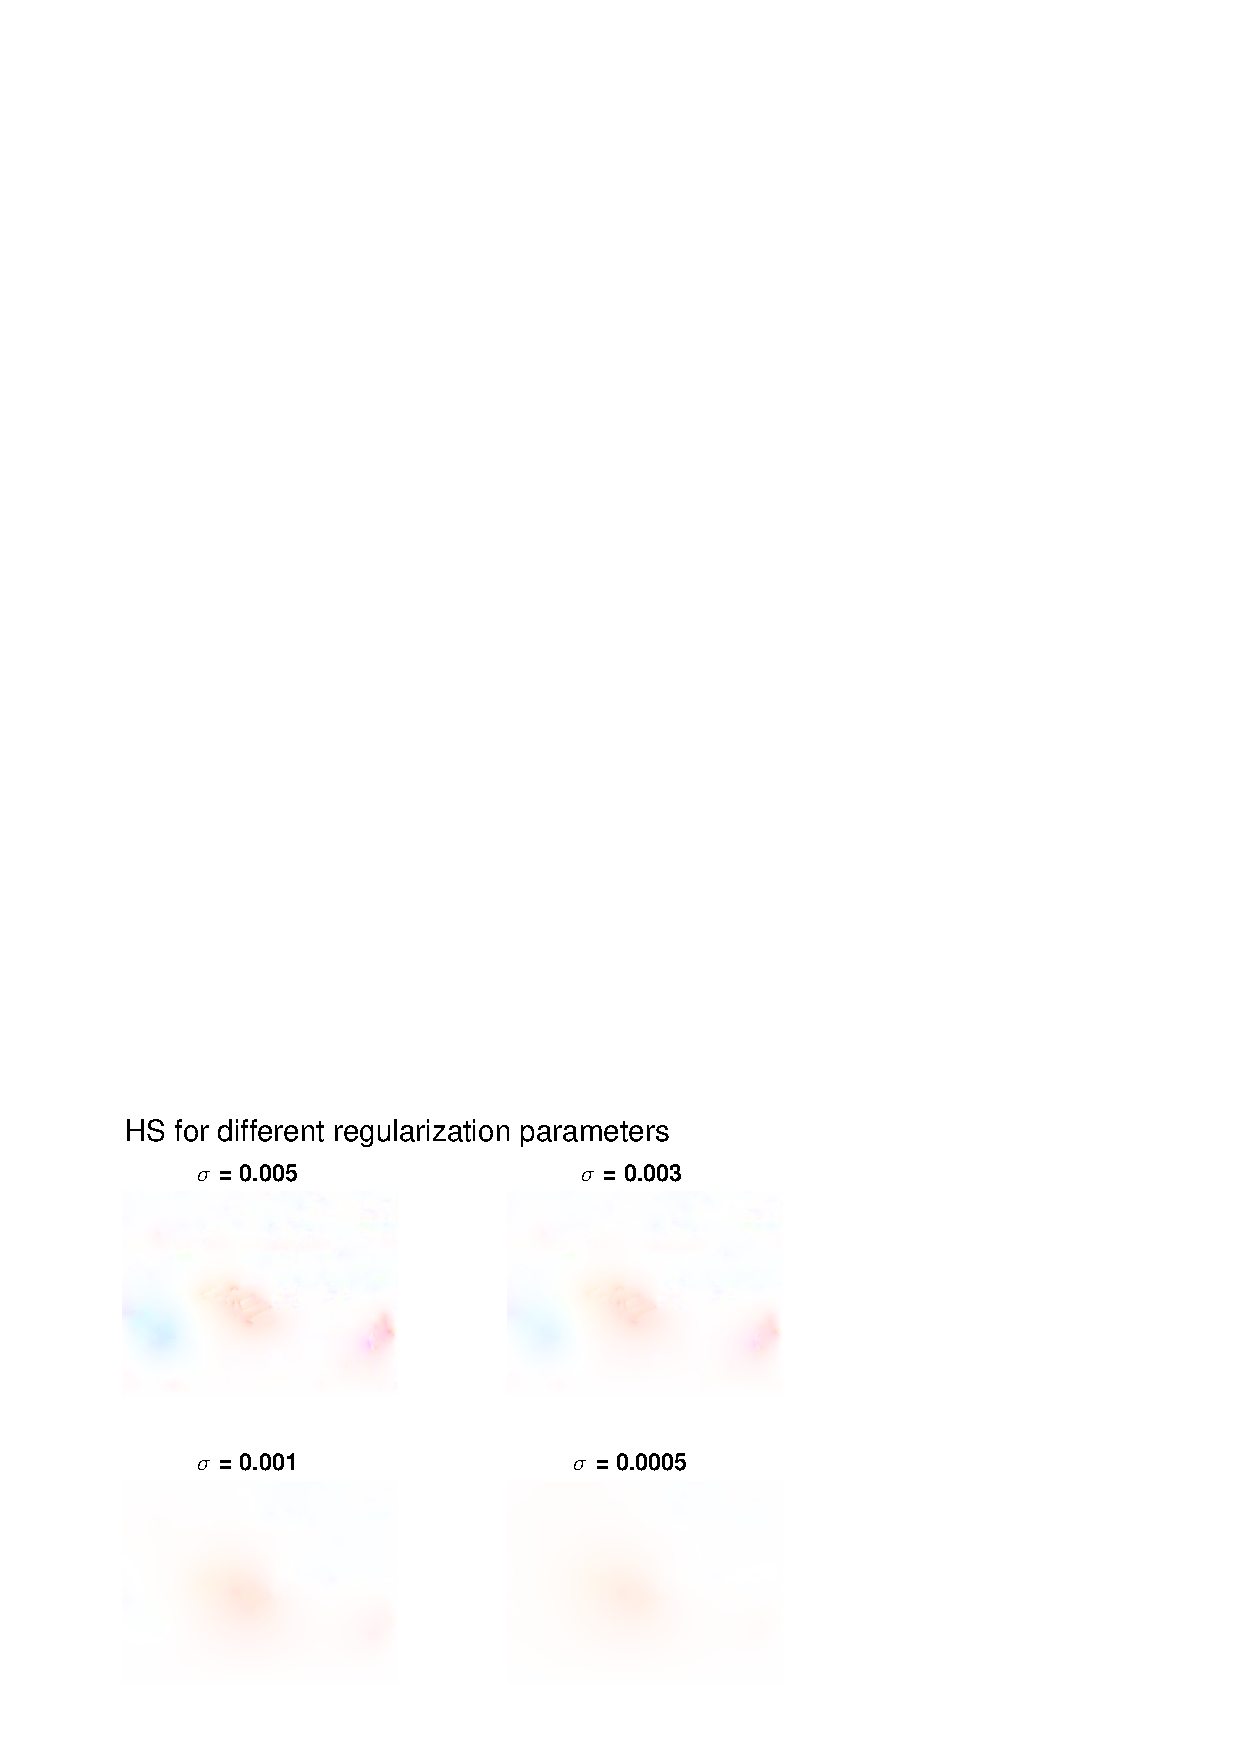
\includegraphics[scale=0.8]{regularizationHS}
    \caption{Different choices for regularization parameter $\sigma$ using the Horn and Schunck algorithm}
    \label{reguHS}
\end{figure}

\begin{figure}
    \centering
    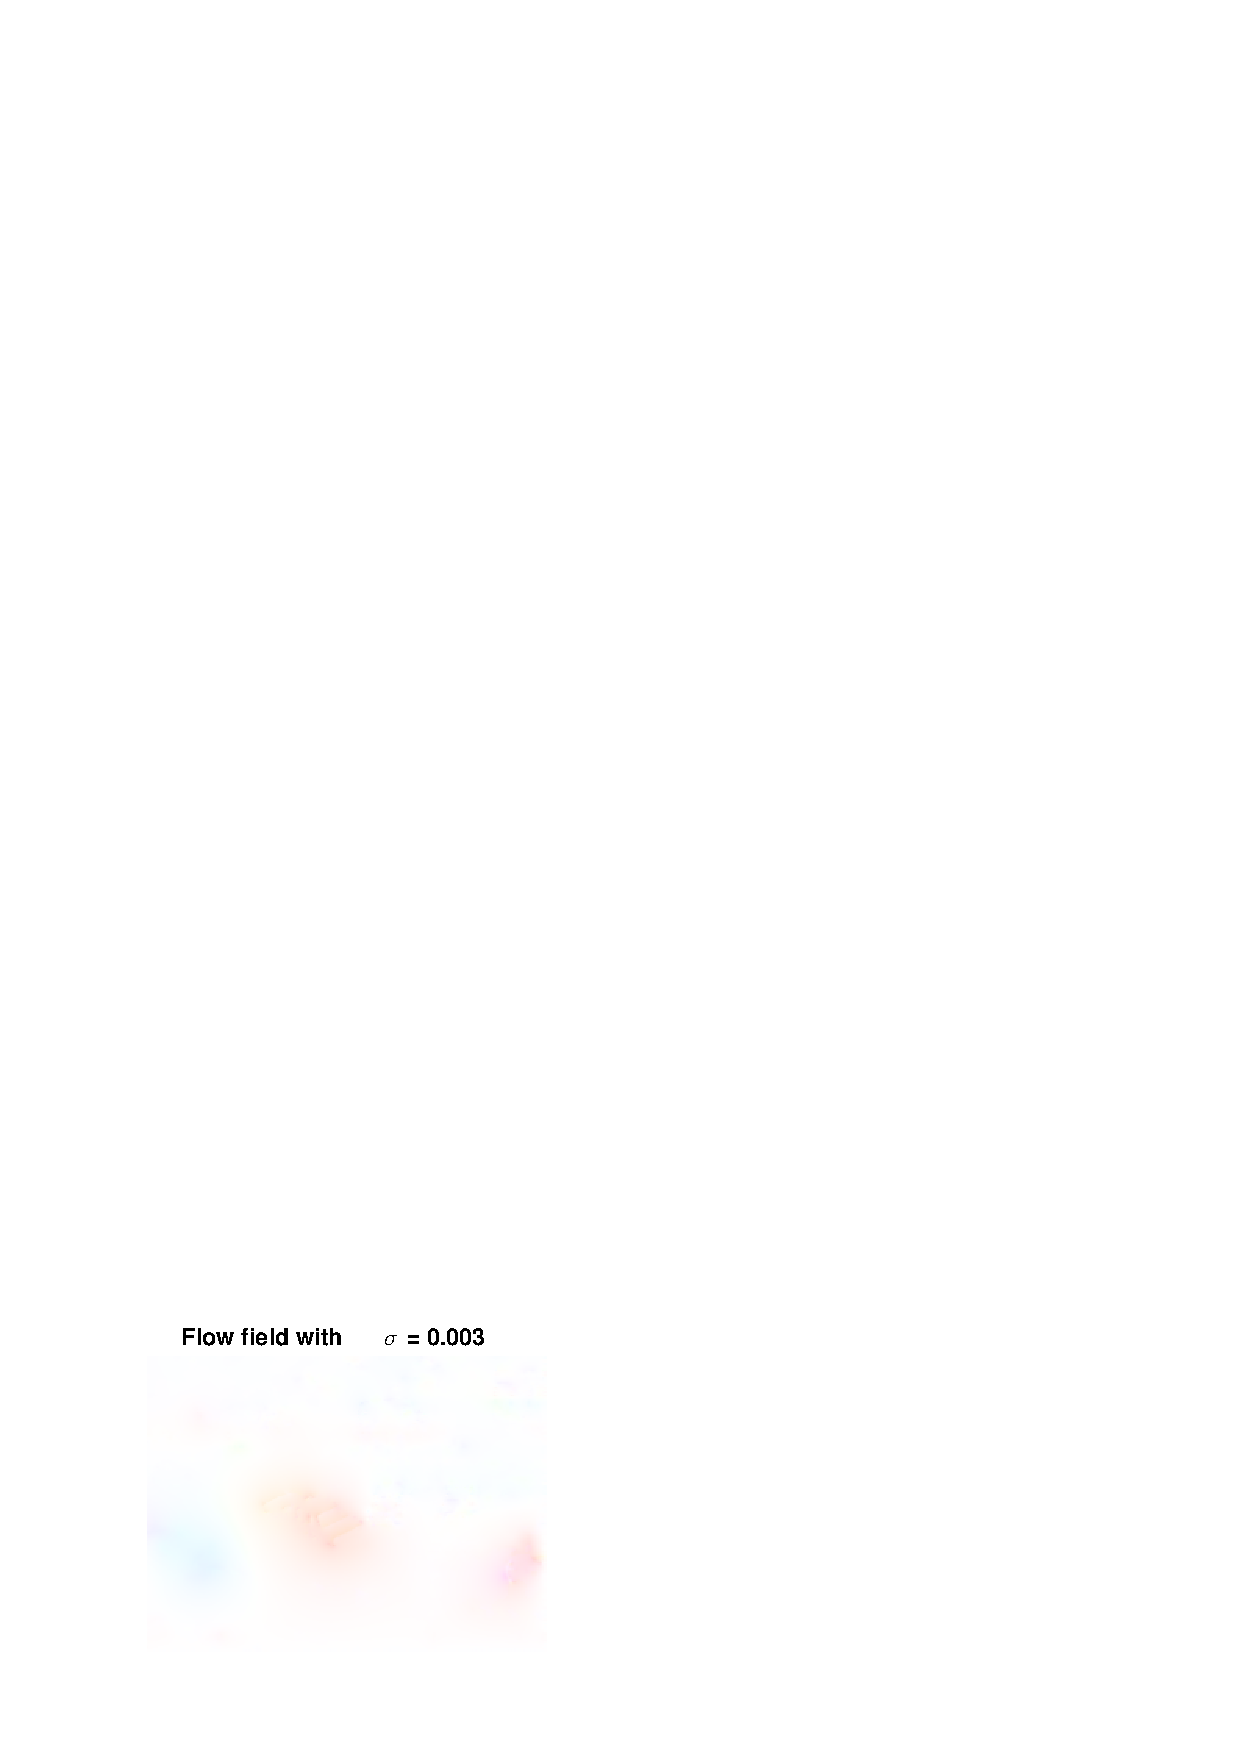
\includegraphics[scale=1]{HSregu}
    \caption{Flow field with $\sigma= 0.003$ using the Horn and Schunck algorithm}
    \label{reguHS_best}
\end{figure}




\section{Anisotropic image-driven regularization}
The homogeneous regularizer of Horn and Schunck smoothes the flow field in all directions. Since we are looking for a flow field describing relative movement of objects, the boundary between objects will not have a smooth flow field unless they are moving at the same relative velocity. Methods that reduce the smoothing across image edges are called image-driven regularization methods. The anisotropic reguralizer of Nagel and Enkelmann (1986) performs smoothing along the image gradients and prevents smoothing across image edges. This is done by introducing a regularised projection matrix $P$, defined as
\begin{align*}
P(\nabla f) = \frac{1}{|\nabla f|^2 + 2 \kappa^2} (\nabla^{\bot} f (\nabla^{\bot})^T + \kappa^2 I),
\end{align*}
where $\nabla^{\bot} f= \left[-\frac{\partial f}{\partial y}, \frac{\partial f}{\partial x}\right]^T$, and $\kappa > 0$ is a regularization parameter. The smoothness term of Nagel and Enkelmann can now be written as the following
\begin{align*}
V_{AI}(\nabla u, \nabla v) = \nabla ^T u P(\nabla f) \nabla u + \nabla ^T v P(\nabla f) \nabla v,
\end{align*}
or written out 
\begin{align*}
V_{AI}(\nabla u, \nabla v) = \frac{\kappa^2}{|\nabla f|^2 + 2 \kappa^2} \left( u_{\textbf{s}_1}^2 + v_{\textbf{s}_1}^2 \right) + \frac{|\nabla f|^2 + \kappa^2}{|\nabla f|^2 + 2 \kappa^2} \left(u_{\textbf{s}_2}^2 + v_{\textbf{s}_2}^2 \right),
\end{align*}
where $\textbf{s}_1 = \frac{\nabla f}{|\nabla f|}$, $\textbf{s}_2 = \frac{\nabla^{\bot} f}{|\nabla f|}$ and $q_{\textbf{s}_i} = \textbf{s}_i^T \nabla u$ for $q = u, v$. That is, $q_{\textbf{s}_i}$ is the directional derivative of $q$ in the direction of the image gradient ($i=1$) or the orthogonal direction ($i=2$). This means that setting $D=P$ in (\ref{EL_regu}) steers the diffusion so that flow vectors are smoothed in the direction of the image gradients.

\subsection{Discretizing the Nagel and Enkelmann smoothness term}
Setting $\Theta=P$ in (\ref{EL_regu}) leads to the following Euler-Lagrange system:
\begin{align*}
\frac{\partial M}{\partial u} - \frac{1}{\sigma^2} \text{div}(P \nabla u) \\
\frac{\partial M}{\partial v} - \frac{1}{\sigma^2} \text{div}(P \nabla v).
\end{align*}
Using the same discretizations for the derivatives as in \ref{sec: disc} we get the following system:
\begin{align*}
(D^T D + \frac{1}{\sigma^2} L^TPL) \textbf{w} = - D^T \textbf{c}.
\end{align*}

\subsection{Results for the anisotropic image-driven regularization}
Experiments were run to find the best regularization parameter in the Nagel and Enkelmann smoothness term. The regularization parameter $\sigma$ found for the Horn and Schunck method is used to regularize the whole smoothness term. The resulting flow field for different choices of the regularization parameter $\kappa$, while keeping $\sigma$ constant, is shown in Figure (\ref{reguNE}). It is seen that choosing $\kappa = 0.8$ gives a fairly good segmentation of the object. Since the values for the gradient from the sobel derivative are relatively high, it is expected to also having to choose a relatively large value for $\kappa$ for sufficient regularization. Figure (\ref{reguNEHS}) compares the anisotropic smoothness term of Nagel and Enkelmann with $\kappa = 0.8$ with the homogeneous smoothness term of Horn and Schunck, both with using regularization parameter $\sigma = 0.003$. 

\begin{figure}
    \centering
    \includegraphics[scale=0.8]{regularizationNE.eps}
    \caption{Different choices for $\kappa$ using the Nagel and Enkelmann smoothness term}
    \label{reguNE}
\end{figure}

\begin{figure}
    \centering
    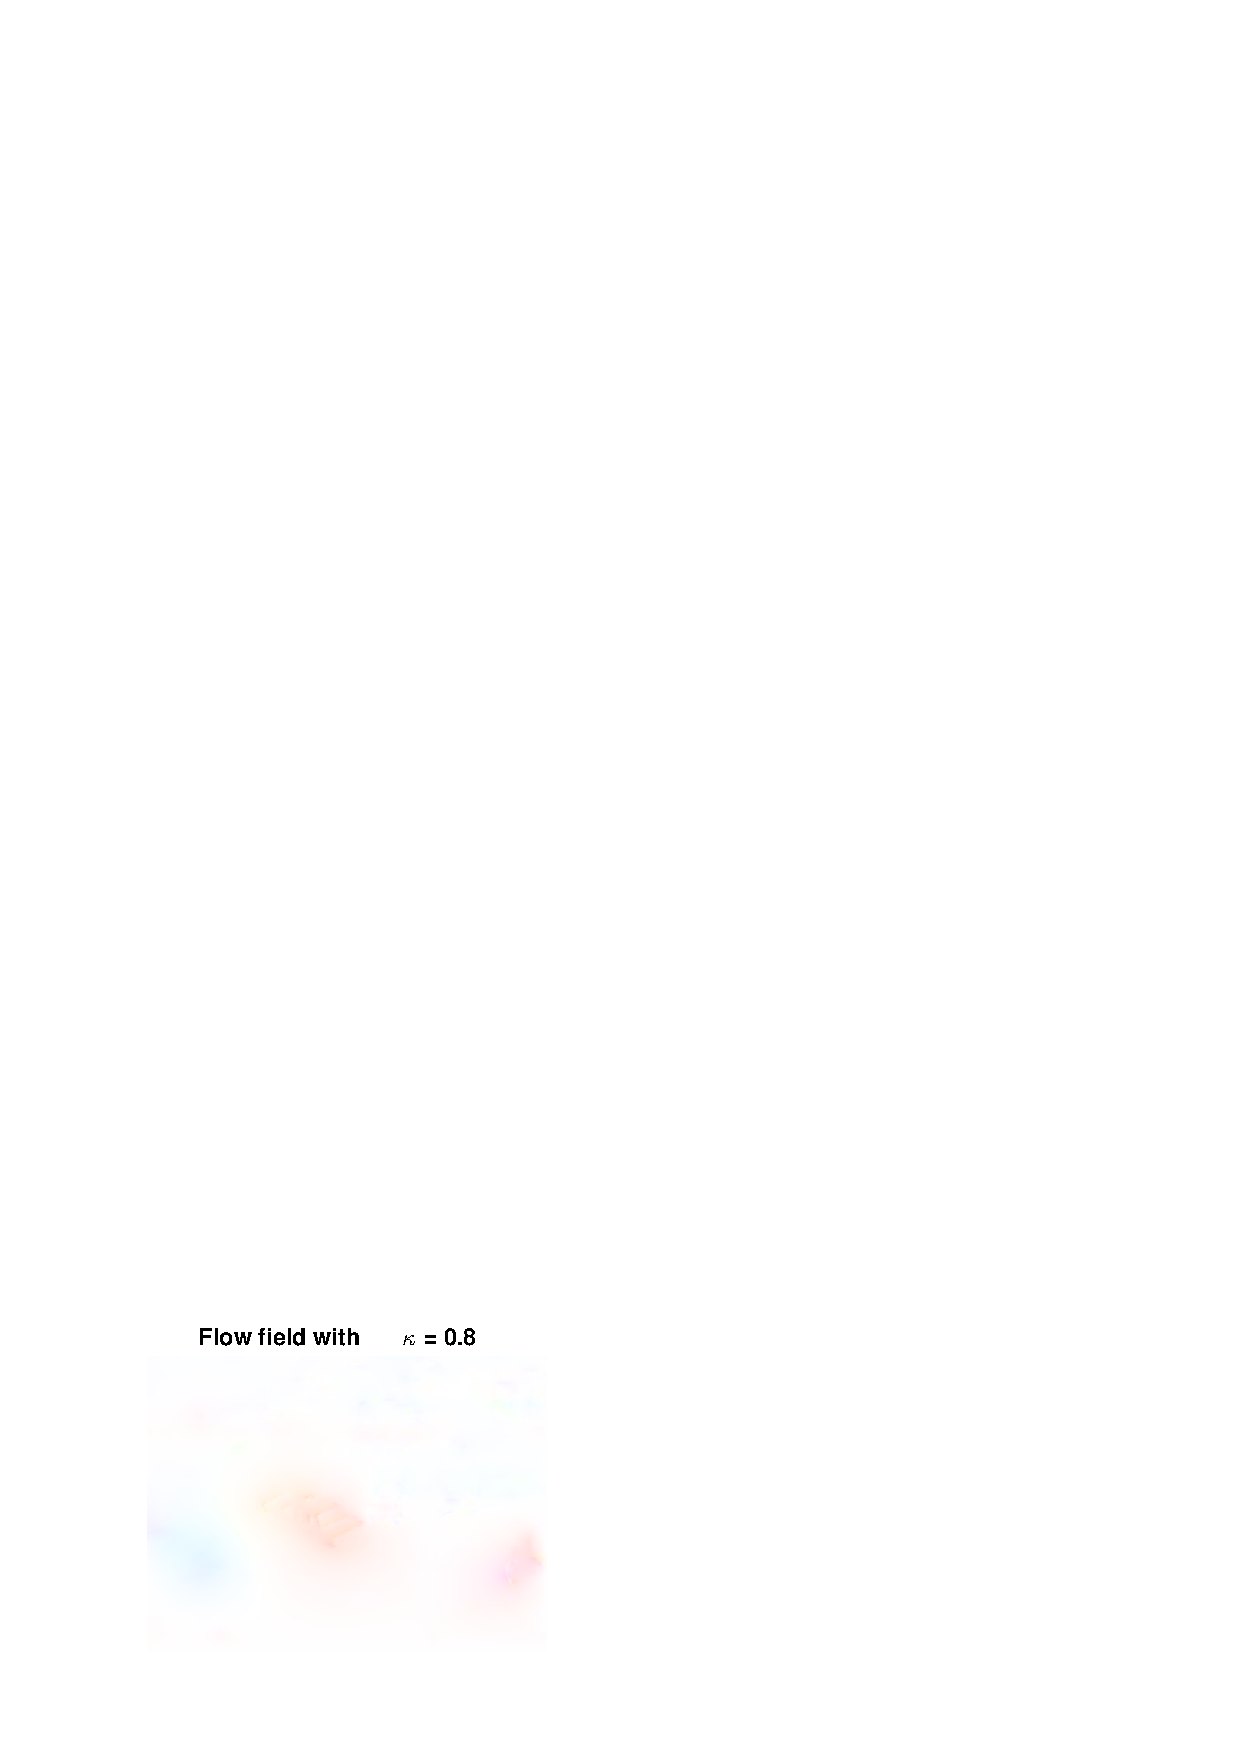
\includegraphics[scale=0.8]{NEregu}
    \caption{Flow field with $\kappa= 0.8$ and $\sigma = 0.003$ using the Nagel and Enkelmann smoothness term.}
    \label{reguNE_best}
\end{figure}

\begin{figure}
    \centering
    \includegraphics[scale=0.8]{reguNEHS.eps}
    \subfloat[\label{NE_best} Anisotropic smoothness term.]{\hspace{.5\linewidth}}
	\subfloat[\label{HS_best} Homogeneous smoothness term.]{\hspace{.5\linewidth}}
	\caption{Comparison of the anisotropic and homogeneous smoothness term for given parameter choices.\label{humans}}
    \label{reguNEHS}
\end{figure}

\section{Isotropic Flow-driven regularization}
One drawback of the image-driven approach to regularization is that there is often a great deal of oversegmentation, since image boundaries are not necessarily flow boundaries. The so called flow-driven methods takes this into account, and decreases smoothing across flow edges instead of image edges. The subquadratic penaliser function of Schulman and Herv (1989) performs a nonlinear isotropic diffusion. The smoothness term can be written as
\begin{align*}
V_{IF}(\nabla u, \nabla v) &= \psi_V \left( |\nabla u|^2 + |\nabla v|^2 \right) \\ 
&= \psi_V \left( u_{\textbf{s}_1}^2 + u_{\textbf{s}_2}^2 + v_{\textbf{s}_1}^2 + v_{\textbf{s}_2}^2 \right),
\end{align*} 
where $\psi_V(s^2)$ is some penaliser function. The contribution to (\ref{EL}) is $\nabla \cdot (\partial_{u_x} V, \partial_{u_y} V)$. Computing the individual components, we get
\begin{align*}
\partial_{u_x} V = 2 \psi_V \left( u_{\textbf{s}_1}^2 + u_{\textbf{s}_2}^2 + v_{\textbf{s}_1}^2 + v_{\textbf{s}_2}^2 \right) u_x \\
\partial_{u_y} V = 2 \psi_V \left( u_{\textbf{s}_1}^2 + u_{\textbf{s}_2}^2 + v_{\textbf{s}_1}^2 + v_{\textbf{s}_2}^2 \right) u_y,
\end{align*}
and equivalent for $(\partial_{v_x} V, \partial_{v_y} V)$. Thus the diffusion matrix of (\ref{EL_regu}) is given as
\begin{align*}
\Theta_{IF} = 2 \psi_V'\left( u_{\textbf{s}_1}^2 + u_{\textbf{s}_2}^2 + v_{\textbf{s}_1}^2 + v_{\textbf{s}_2}^2 \right) I,
\end{align*}
where $I$ is the identity matrix, which is seen to be a function of the flow gradient. As a convex penaliser, Cohen (1993) suggested the following total variation regulariser:
\begin{align*}
\psi_V(s^2) = \sqrt{s^2 + \epsilon^2},
\end{align*} 
which gives
\begin{align*}
\psi_V'(s^2) = \frac{1}{2 \sqrt{s^2 + \epsilon^2}}.
\end{align*}
This penaliser function results in the following Euler-Lagrange system
\begin{equation}
\begin{aligned}
\label{EL_LD}
\partial_u M - \frac{1}{\sigma^2} \left(\frac{\partial}{\partial x}\left[ \frac{u_x}{\sqrt{|\nabla u|^2 + |\nabla v|^2}} \right] + \frac{\partial}{\partial y} \left[ \frac{u_y}{\sqrt{|\nabla u|^2 + |\nabla v|^2}} \right] \right) = 0 \\
\partial_v M - \frac{1}{\sigma^2} \left(\frac{\partial}{\partial x}\left[ \frac{v_x}{\sqrt{|\nabla u|^2 + |\nabla v|^2}} \right] + \frac{\partial}{\partial y} \left[ \frac{v_y}{\sqrt{|\nabla u|^2 + |\nabla v|^2}} \right] \right) = 0,
\end{aligned}
\end{equation}
which is clearly a non-linear system.


\subsection{The Lagged Diffusivity Fixed Point Method}
The non-linear system (\ref{EL_LD}) can be solved using the method of lagged diffusivity, which is a fixed point scheme that can be traced back to Weiszfeld's method of minimizing Euclidean lengths, and for which global and linear convergence can be proven (Chan et. al. 1999). From (\ref{EL_LD}) we can define the fixed point method as
\begin{align*}
\partial_{u^{k+1}} M - \frac{1}{\sigma^2} \left(\frac{\partial}{\partial x}\left[ \frac{u^{k+1}_x}{\sqrt{|\nabla u^k|^2 + |\nabla v^k|^2}} \right] + \frac{\partial}{\partial y} \left[ \frac{u^{k+1}_y}{\sqrt{|\nabla u^k|^2 + |\nabla v^k|^2}} \right] \right) &= 0 \\
\partial_{v^{k+1}} M - \frac{1}{\sigma^2} \left(\frac{\partial}{\partial x}\left[ \frac{v^{k+1}_x}{\sqrt{|\nabla u^k|^2 + |\nabla v^k|^2}} \right] + \frac{\partial}{\partial y} \left[ \frac{v^{k+1}_y}{\sqrt{|\nabla u^k|^2 + |\nabla v^k|^2}} \right] \right) &= 0,
\end{align*}
where we solve for $u^{k+1}$ and $v^{k+1}$ given $u^k$ and $v^k$ from the previous iteration. This is a linear system in each iteration, and it can be solved in the same manner as the previous methods. The system to be solved at iteration $k+1$ is
\begin{align*}
(D^T D + \frac{1}{\sigma^2} L^T\Theta^{k}L) \textbf{w}^{k+1} = - D^T \textbf{c},
\end{align*}
where $\Theta^k$ is the following 4mn-by-4mn diagonal block matrix
\begin{align*}
\Theta^k = \left[
\begin{array}{c|c|c|c}
\chi^k & 0 & 0 & 0 \\ \hline
0 & \chi^k & 0 & 0 \\ \hline
0 & 0 & \chi^k & 0 \\ \hline
0 & 0 & 0 & \chi^k
\end{array}
\right].
\end{align*}
The submatrix $\chi^k$ is the mn-by-mn diagonal matrix with the values 
\begin{align*}
\chi^k_i = 2 \psi_V'\left( \left[u^k_{\textbf{s}_1}(x^i)\right]^2 + \left[u^k_{\textbf{s}_2}(x^i)\right]^2 + \left[v^k_{\textbf{s}_1}(x^i)\right]^2 + \left[v^k_{\textbf{s}_2}(x^i)\right]^2 \right)
\end{align*}
along its diagonal.
  

\begin{thebibliography}{}

\bibitem{Chan}
Chan, T. and Mulet, P. (1999) On the convergence of the lagged diffusivity fixed point method in total variation image restoration. \emph{SIAM Journal of Numerical Analysis} (Vol. 36, No. 2, pp 354-367)

\bibitem{Cohen}
Cohen, I. (1993). Nonlinear variational method for optical flow computation. \emph{Proceedings. Eighth Scandinavian conference on Image Analysis} (Vol. 1, pp. 523–530). Norway, Tromsø.

\bibitem{CH}
Courant, R. and Hilbert, D. (1953). Methods of Mathematical Physics. Vol. I (First English ed.), Interscience Publishers, New York

\bibitem{Courant}
Courant, R. (1947). Differential and Integral Calculus, Vol. II, 2nd edition, Interscience Publishers, New York


\bibitem{HS}
Horn, B. and Schunck, B. (1981). Determining optical flow. \emph{Artificial Intelligence}, 17, 185-203.

\bibitem{NE}
Nagel, H. and Enkelmann, W. (1986). An investigation of smoothness constraints for the estimation of displacement vector fields from image sequences. \emph{IEEE Transactions on Pattern Analysis and Machine Intelligence}, 8, 565-593

\bibitem{SH}
Shulman, D. and Hervé, J. (1989). Regularization of discontinuous flow fields. \emph{Proceedings. Workshop on Visual Motion} (pp. 81–86). Irvine: IEEE Computer Society Press.

\bibitem{OFH}
Zimmer, H., Bruhn, A., Weickert, J. (2011). Optic Flow in Harmony \emph{International Journal of Computer Vision}, 93, 368-388


\end{thebibliography}


\end{document}

